\chapter{Beispiele} \label{c:beispiele}

Im Kapitel Beispiele (siehe \autoref{c:beispiele}) werden die möglichen Funktionen und\index{und} Möglichkeiten dies LaTeX-Dokuments demonstriert.

\section{Quelltext}

Nachfolgend der \autoref{lst:helloworld}.

\begin{lstlisting}[caption={Hello World}, captionpos=b, label={lst:helloworld}]
/**
* The HelloWorldApp class implements an application that
* simply prints "Hello World!" to standard output.
*/
class HelloWorldApp {
	public static void main(String[] args) {
		System.out.println("Hello World!"); // Display the string.
	}
}
\end{lstlisting}

\section{Bild}

\begin{wrapfigure}{R}{0.5\textwidth}
	\centering
	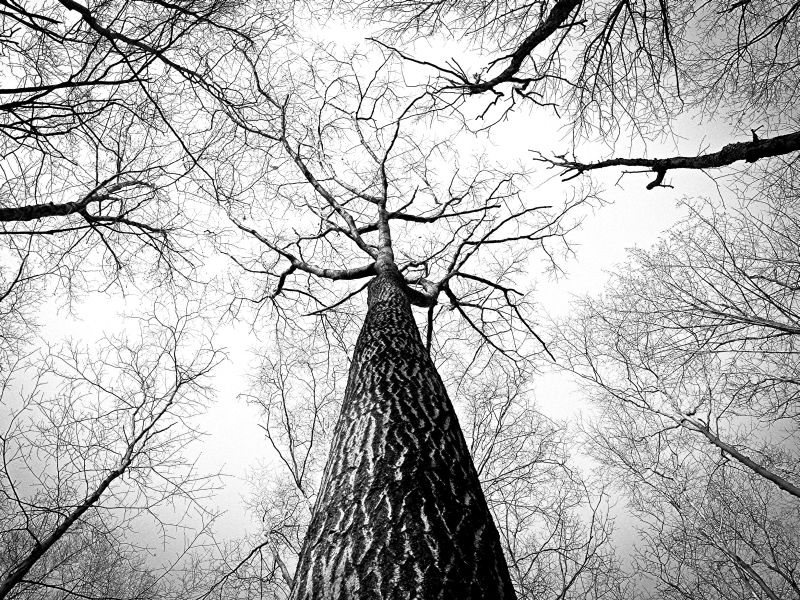
\includegraphics[width=0.5\textwidth]{resources/example}
	\caption{Beispielbild {\cite{PEXELS2015}}}
\end{wrapfigure}

Die rechts zu sehende Grafik demonstriert die Möglichkeiten des Paketes \glqq wrapfig\grqq . Grafiken innerhalb einer \glqq wrapfigure\grqq{} können entweder links oder rechts von Text umlaufen werden.

Die nachfolgende \autoref{img:beispielbild} demonstriert die Darstellung\index{Darstellung} eines \glqq *.jpg\grqq{} Bildes innerhalb des Textes (beim Einfügen kann auf die Endung verzichtet werden, solange der Name einzigartig ist). Zusätzlich enthält dieses einen Untertitel der über das bereits verwendete Label verlinkt werden kann. Der Untertitel\index{Untertitel} erscheint im \gls{abbvz}.

\section{Text Formatierungen und sonstiges}
Dieser Text enthält eine Fußnote\footnote{Fußnoten sind Anmerkungen, die im Druck-Layout aus dem Fließtext ausgelagert werden, um den Text flüssig lesbar zu gestalten.}.

\subsection{Listen}
Listen könne sowohl mit Bullet points als auch mit Zahlen erstellt werden
\begin{itemize}
	\item Eine Liste mit Bullet points
	\item Ein weiteres Element
\end{itemize}

\begin{enumerate}
	\item Eine Liste mit Zahlen
	\item Ein weiteres Element
\end{enumerate}

\subsection{Text Hervorhebungen}
\begin{quote}
	The problem with internet quotes is that you can't always depend on their accuracy \par\raggedleft--- \textup{Abraham Lincoln, 1864}
\end{quote}

"Inspirierende Zitate können mit epigraph eingefügt werden
\epigraph{The problem with internet quotes is that you can't always depend on their accuracy}{Abraham Lincoln, 1864}

Seitenumbrüche können nur direkt nach Text geschrieben werden, sonst lässt sich das Latex nicht mehr compilieren.
\\

\begin{figure}[H]
	\centering
	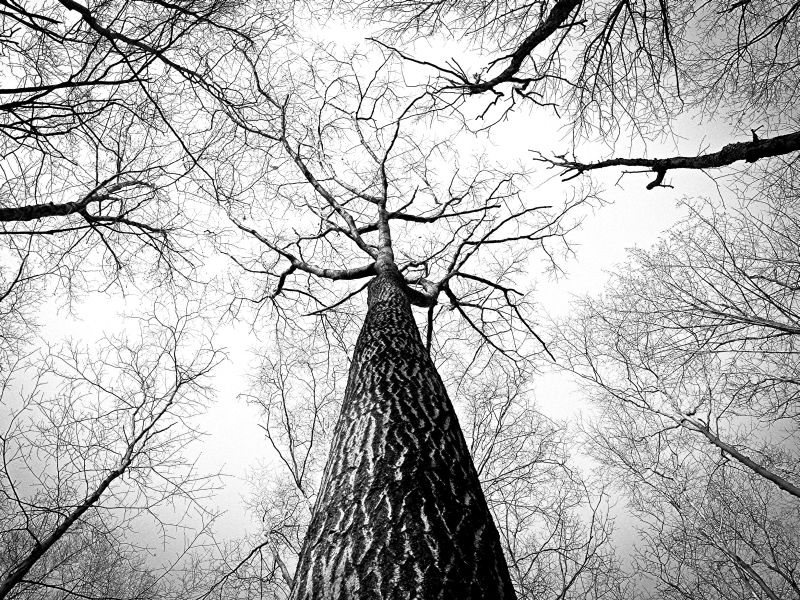
\includegraphics[width=0.7\textwidth]{resources/example}
	\caption{Beispielbild {\cite{PEXELS2015}}}
	\label{img:beispielbild}
\end{figure}

\section{Tabelle}

Nachfolgend \autoref{tbl:DigitalesZertifikat}.

\begin{table}[H]
	\begin{center}
		\renewcommand{\arraystretch}{1.3}
		\begin{tabular}{|l|}
			\hline
			\textbf{Inhaber:}\\
			Alice \\ \hline
			\textbf{Peer (Ersteller):}\\
			Bob \\ \hline
			\textbf{Öffentlicher Schlüssel des Inhabers:}\\
			F2 D2 0E ED FA 4E 9E 0A F2 DD 23 8A 32 44 F3 E9 \\ \hline
			\textbf{Gültigkeit:}\\
			2015-07-01 – 2016-06-30 \\ \hline
		\end{tabular}
	\end{center}
	\caption{Digitales Zertifikat}
	\label{tbl:DigitalesZertifikat}
\end{table}

\section{Literaturverweis}

Weil für die alte\index{alte} und die neue Rechtschreibung verschiedene Trennregeln\index{Trennregeln} gelten, sind Deutsch mit alter Rechtschreibung und Deutsch mit neuer Rechtschreibung zwei verschiedene Sprachen (\cite{Knappen2009}, S. 192).

\section{Onlineverweise}

Siehe Google.de \cite{Google2015}.

\section{Glossar}
Der Glossar enthält die Beschreibung verwendeter Begriffe für das bessere Verständnis gegenüber dem Leser. Beispiele sind: \gls{berlin}, \gls{outsourcing}, \gls{asp}, \gls{policy} und \gls{pcie}.

\section{Abkürzungsverzeichnis}
Das Abkürzungsverzeichnis listet alle verwendeten Abkürzungen auf. Einige Beispiele sind \gls{sas}, \gls{cd}, \gls{lan} und \gls{iso}. Die erneute Verwendung zeigt nur noch die Abkürzung: \gls{sas}, \gls{cd}, \gls{lan} und\index{und} \gls{iso}.